\section*{\uppercase{Appendix}}

Table~\ref{tab:pairs} lists the 48 pairs used in this work. The examples in Section~\ref{sec:results} use garments 01474 (stripe), 00205 (floral) and 02268 (lettering).
\\
\begin{table*}[t]
  \centering
  \caption{The 48 \vitonhd test pairs, given as person\,/\,garment image ID (the suffix \texttt{\_00} of every file name is left out).}
  \label{tab:pairs}
  \footnotesize
  \begin{tabular}{lcccccc}
  \toprule
  Category & \multicolumn{6}{c}{Person\,/\,garment} \\
  \midrule
  Solid & 02527\,/\,00006 & 05627\,/\,14675 & 01713\,/\,10087 & 06333\,/\,07247 & 00599\,/\,04395 & 05170\,/\,12106 \\
  Lettering & 02116\,/\,00126 & 12006\,/\,03838 & 09104\,/\,14673 & 07278\,/\,02268 & 07190\,/\,13987 & 09305\,/\,11638 \\
  Graphic & 12749\,/\,05537 & 13351\,/\,04450 & 05703\,/\,07241 & 09236\,/\,00396 & 12178\,/\,07180 & 02973\,/\,13975 \\
  Stripe & 13758\,/\,00286 & 09204\,/\,01474 & 03475\,/\,09520 & 01670\,/\,03267 & 07309\,/\,04818 & 11390\,/\,03003 \\
  Floral & 14674\,/\,00205 & 00259\,/\,01689 & 10709\,/\,08871 & 05544\,/\,05056 & 03975\,/\,10885 & 14586\,/\,03126 \\
  Dot & 10374\,/\,00095 & 07202\,/\,04137 & 14134\,/\,06802 & 11351\,/\,06196 & 14572\,/\,04972 & 10078\,/\,11102 \\
  Check & 02991\,/\,07796 & 07319\,/\,07050 & 08977\,/\,03413 & 02054\,/\,06379 & 11632\,/\,05935 & 08690\,/\,13730 \\
  Structural & 11158\,/\,00034 & 01755\,/\,01641 & 04545\,/\,12186 & 06423\,/\,03407 & 01630\,/\,01403 & 05667\,/\,00463 \\
  \bottomrule
  \end{tabular}
\end{table*}

\noindent Figure~\ref{fig:x0_strip_appendix} shows the decoded estimate $\hat{x}_0$ for one pair of each category that is not shown in Section~\ref{sec:results}. For each category we chose the pair whose scores at step 10 are closest to the category mean, so these pairs are typical rather than the clearest examples. The only exception is (f), a floral print on which \ootd is also late.
\\ \\
\noindent The pairs show the same order as the striped and floral examples in the main text. In every pair the person and the silhouette of the garment are in place by step 5. On the plain garment (a), the colour still changes after that: \catvton starts with a more saturated green and \idm with a blue that only turns into the final teal around step 20. On the graphic print (b), \catvton leaves the region below the print blurred until step 10, while \ootd and \idm show the print and the skirt from step 5. The ruffle on the structural top (c) appears only after step 20 in all three models, although the colour and the outline of the top are fixed much earlier. The dots (d) and the check (e) follow the stripes: \ootd shows them from step 1, \idm from around step 10 and \catvton from around step 20. On the check, \idm also starts with a blue that is not in the garment. The floral print (f) is a case where none of the models shows the flowers before step 20, which agrees with the low texture AUC of floral prints in \ootd.

\begin{figure*}[t]
  \centering
  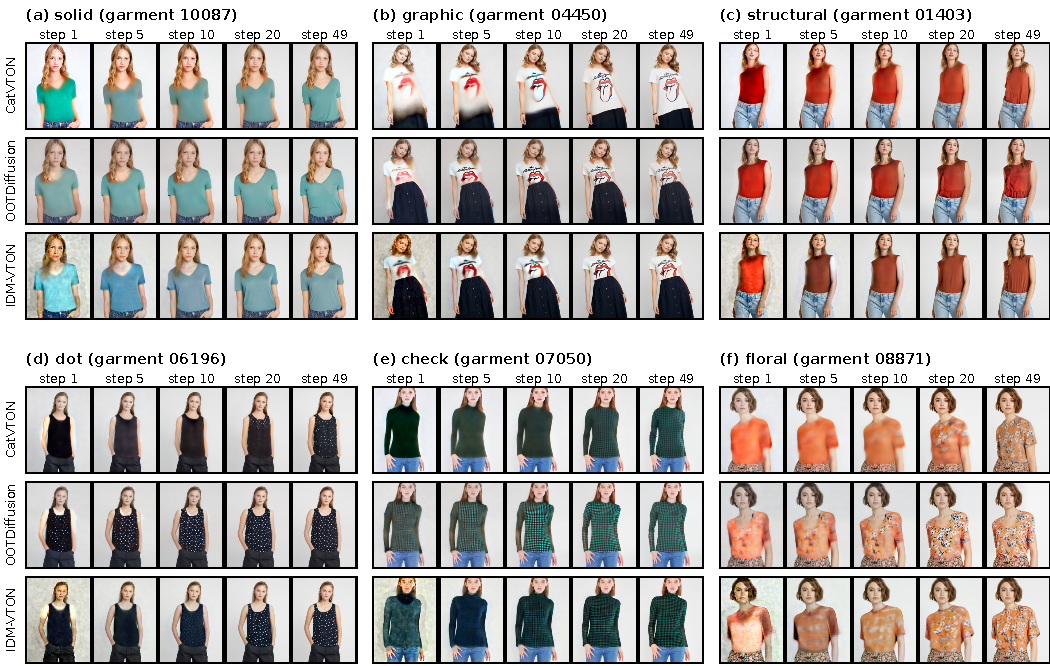
\includegraphics[width=\textwidth]{figures/x0_strip_appendix.pdf}
  \caption{Decoded estimate $\hat{x}_0$ at five steps for one pair of each remaining category: (a) solid, (b) graphic, (c) structural, (d) dot, (e) check and (f) a second floral print.}
  \label{fig:x0_strip_appendix}
\end{figure*}
